\documentclass[12pt,a4paper,oneside]{article}
\usepackage{graphicx}
\usepackage{float} %for [H]


\usepackage{titlepic}
\usepackage[utf8]{inputenc}
\usepackage[left=1.1in,right=1.1in, top=1in, bottom= 1in]{geometry}
\usepackage[none]{hyphenat} % Avoids to go out of margin
\usepackage{subfiles}

% Font size of figure smaller than normal size:
\usepackage{caption}
\captionsetup[figure]{font=small}
\linespread{1.2}

% --------------------------------------------- %

\title{Homework 1}	                                    % Title
\author{Flavio Maiorana 2051396}				                % Authors separated by \\
\date{\today}								    % Date

\makeatletter
\let\thetitle\@title
\let\theauthor\@author
\let\thedate\@date
\makeatother

\begin{document}

\begin{titlepage}
	\centering
    \vspace*{0.5 cm}
    
\includegraphics[scale = 0.75]{figures/SapienzaLogo.pdf}\\[1.0 cm]	% University Logo

    % \vspace*{-0.4cm}
    % \textsc{\large DIAG}\\[2.0 cm]	% Department Name
    % \vspace*{1cm}

    { \fontsize{20.74pt}{18.5pt}\selectfont\bfseries \thetitle \par } % Title

    \vspace*{0.25cm}
    \textsc{\Large Machine Learning}\\[0.5 cm] % Course Name

    \vspace*{2.6cm}
	% \begin{minipage}{0.4\textwidth} % 0.4
	% 	\begin{flushleft} \large
	% 		\textbf{Professors:}\\
	% 		Professor Name\\
	% 	\end{flushleft}
	% \end{minipage}~
	\begin{minipage}{0.3\textwidth} %0.4
		\begin{flushright} \large
		\begin{minipage}{1\textwidth}
		\begin{flushleft} \large
			\textbf{Students:} \\
			\theauthor
        \end{flushleft}
        \end{minipage}
		\end{flushright}
	\end{minipage}\\[3.85 cm]

    \vspace{2cm}
    \rule{\linewidth}{0.2 mm} \\[0.3 cm]
    \vspace*{-0.2cm}
    Academic Year 2023/2024
\end{titlepage}
\newpage

When approaching a classification problem, the steps to be followed
usually start from looking at the dataset and eventually doing some actions on
it even before "cranking up" the learning algorithm.

\section{Data visualization and preprocessing}

First of all, it could be useful to gain some insight one how the dataaset is
made.

\begin{verbatim}[Dataset 1]
    N Examples: 50000
    N Inputs: 100
    N Classes: 10 [0 1 2 3 4 5 6 7 8 9]
     - Class 0: 5000 (10.0)
     - Class 1: 5000 (10.0)
     - Class 2: 5000 (10.0)
     - Class 3: 5000 (10.0)
     - Class 4: 5000 (10.0)
     - Class 5: 5000 (10.0)
     - Class 6: 5000 (10.0)
     - Class 7: 5000 (10.0)
     - Class 8: 5000 (10.0)
     - Class 9: 5000 (10.0)
\end{verbatim}

\begin{verbatim}[Dataset 2]
    N Examples: 50000
    N Inputs: 1000
    N Classes: 10 [0 1 2 3 4 5 6 7 8 9]
     - Class 0: 5000 (10.0)
     - Class 1: 5000 (10.0)
     - Class 2: 5000 (10.0)
     - Class 3: 5000 (10.0)
     - Class 4: 5000 (10.0)
     - Class 5: 5000 (10.0)
     - Class 6: 5000 (10.0)
     - Class 7: 5000 (10.0)
     - Class 8: 5000 (10.0)
     - Class 9: 5000 (10.0)
\end{verbatim}

Some comments: both datasets have examples pertaining 10 different Classes, The
number of examples is pretty high and Both datasets are perfectly balanced

\begin{figure}[H]
    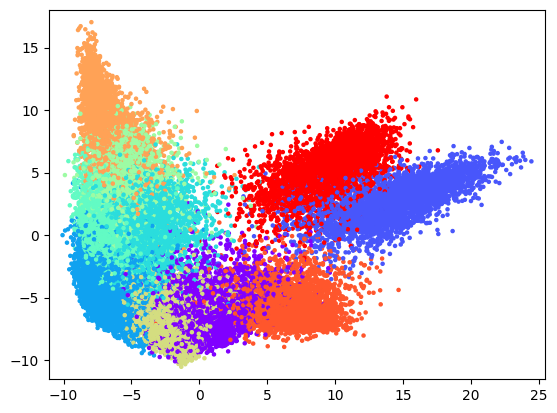
\includegraphics{figures/dataset1.png}
    \caption{Dataset 1 with PCA}
\end{figure}

\begin{figure}[H]
    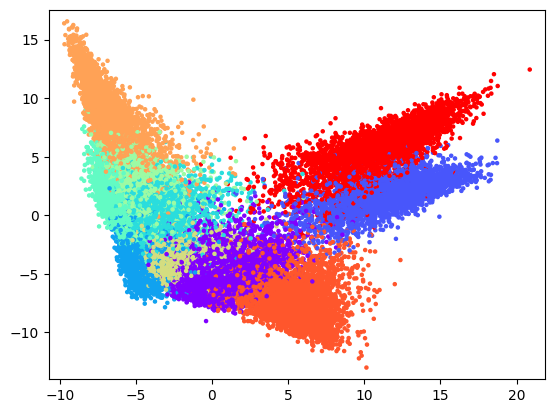
\includegraphics{figures/dataset2.png}
    \caption{Dataset 2 with PCA}
\end{figure}

\newpage

After that, one could want to graphically visualize the data in order to be able
to spot some peculiarities of it by just literally looking at it. Although, the
first problem we confront with using this specific tyoe of dataset is the number
of features. To that end, dimensionality reduction could be used to visually
represent the dataset in two dimensions. As we can see from these two plots, the
samples of each class are pretty much higly concentrated around the mean, so the
variance is low, and also, apparently, the number of (isolated) outliers is
pretty low. This could be facilitating the learning algorithm. One thing that
could make our life more difficult is the fact that, at least apparently
based one this 2D plot, some classes are overlapping, which could cause certain
samples from two slightly overlapping classes to be exchanged.

Then, one could preprocess the dataset by scaling the features. That is usually
done to ensure that the features are equally scaled, since they could be of
different unit measures. That helps learning algorithms to optimize the learning
process. Specifically, we scale the features in order for them to be of mean 0
and variance 1. As an example, one could look at the first sample of Dataset1
and observe that the values range from 0 to ca. 4 (no negative values). Instead
after applying the feature scaling, also negative values appear, and the range
of values is between -1.15 and 1.15 approximatively.

\subsection{Preprocessing for evaluation}

Last but not least, the dataset has to be treated in order to sensibly train and
test any training algorithm. To that end, one could use a train test split.
Specifically, the used percentage is 0.7 for the train split and 0.3 for the
test split. During the training phase, the learning algorithm will be exposed
only to the train split, trying to optimize some function based only on that
data. After that, the score will be evaluated on the test data. This allows the
training algorithm to evaluate its performance on previously unseen samples. One
could also use k-fold cross validation to assess the performance of different
learning algorithms, especially to compare them with the appropriate metrics.


\section{Models}

Different approaches can be used to solve this problem. We will treat mainly 4
models: KNN, SVM (linear and nonlinear), Gaussian Naive Bayes and Softmax
Regression. They will be compared based on the same train-test split.

\subsection{KNN}

First, a non-parametric method could be used, but mainly as a baseline,
especially because, with a big input space (for decision trees) or a big number
of samples (for knn), it would behave poorly from the computational point of
view. The latters happens because with non-parametric instance based methods we
have to store the entire training set in order to classify a new sample. Anyway,
KNN has been used together with a hyperparameter search. Shortly, KNN predicts
the class of a sample by looking at the k neirest neighbors with an
apprioprately chosen distance metrics. Also, as the number of neighbors rises,
the computational cost of inference rises too.

For this learning algorithm, two different hyperparameter configurations were
tried: the first with 5 neighbors, uniform weights for each sample and euclidean
distance as metric. With this configuration we obtain the following evaluation
data for the first dataset: 

\begin{verbatim} [Dataset 1]
    Train Accuracy:  0.9890285730361938
    Test Accuracy:  0.9886000156402588
              precision    recall  f1-score   support

           0      0.998     0.993     0.995      1551
           1      0.997     0.995     0.996      1468
           2      0.988     0.990     0.989      1505
           3      0.960     0.978     0.969      1465
           4      0.983     0.990     0.987      1483
           5      0.979     0.964     0.971      1592
           6      0.997     0.991     0.994      1536
           7      0.992     0.991     0.992      1462
           8      0.995     0.999     0.997      1484
           9      0.995     0.997     0.996      1454

    accuracy                          0.989     15000
   macro avg      0.989     0.989     0.989     15000
weighted avg      0.989     0.989     0.989     15000
\end{verbatim}

\begin{figure}[H]
    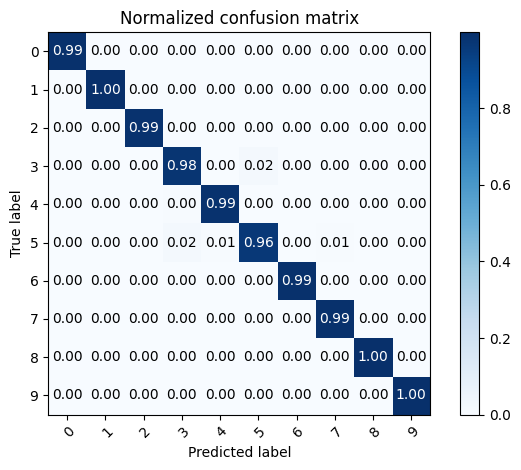
\includegraphics{figures/knn_plain_cm.png}
    \caption{Knn Dataset 1}
\end{figure}

As we can see, classes 3 and 5 are the ones which get the lowest scores since
they get confused between each other. We see that from the fact that they have
lower precision and recall scores, namely they tend to be associated to samples
which are false negatives or false positives. Most probably that depends on how
the dataset is made, namely the overlap between the two classes.

Instead for the second dataset we have:

\begin{verbatim}[Dataset 2]
    Train Accuracy:  0.9764571189880371
    Test Accuracy:  0.9701333045959473
              precision    recall  f1-score   support

           0      0.984     0.981     0.983      1551
           1      0.986     0.994     0.990      1468
           2      0.968     0.974     0.971      1505
           3      0.902     0.932     0.917      1465
           4      0.965     0.972     0.968      1483
           5      0.947     0.914     0.930      1592
           6      0.988     0.977     0.983      1536
           7      0.979     0.980     0.979      1462
           8      0.991     0.993     0.992      1484
           9      0.994     0.988     0.991      1454

    accuracy                          0.970     15000
   macro avg      0.970     0.970     0.970     15000
weighted avg      0.970     0.970     0.970     15000
\end{verbatim}

The performance is similar to the one with the first dataset, but a little bit
lower. That is obviously due to the higher number of input features.





\bibliographystyle{unsrt}
\bibliography{ref}
\nocite{*}  % to include references which were not cited

\end{document}